\chapter{Zagadnienia merytoryczne}
\label{cha:pierwszyDokument}

Przed przystąpieniem do opisywania przebiegu zrealizowanych prac niezbędne jest przytoczenie pewnego wstępu merytorycznego, który to przybliży najistotniejsze kwestie teoretyczne omawiane w dalszych rozdziałach niniejszego tekstu. Podstawowe opisanie kluczowych zagadnień jest zatem niezbędne by stworzyć zarys całości projektu i tym samym przysłużyć się ku dokładnemu jego zrozumieniu.

%---------------------------------------------------------------------------
\section{Wykorzystywany robot}

Jak wspomniano we wstępie wykorzystywane urządzenie było robotem stworzonym na potrzeby zrealizowanej pracy inżynierskiej. Była to konstrukcja w konfiguracji RRR. Łącznie manipulator wyposażony był w 5 stopni swobody, a co za tym idzie 5 osi obrotu. Na ostatnim ramieniu umieszczony został chwytak, pozwalający na łapanie niewielkich przedmiotów. Poniższe zdjęcie przedstawia pierwotny wygląd urządzenia tj. zanim jeszcze przystąpiono do implementacji kontrolera i związanych z nim zmian - rysunek \ref{fig:1}.

Urządzenie posiada napęd w postaci silników krokowych typu Nema 17, sterowanych z poziomu mikrokontrolera STM32F303 poprzez stepsticki - czyli niewielkie sterowniki wspomnianych silników. Wszystkie części strukturowe konstrukcji zostały wydrukowane na drukarce 3D. Koncepcja robota zakładała umieszczenie silników na obrotowej wieży, a dalej poprzez paski zębate przekazanie napędu do poszczególnych osi obrotu. Oczywiście nie wszystkie silniki umieszczono na wspomnianej wieży. Dwa pozostałe są kolejno w podstawie oraz na końcu ramienia drugiego. Chwytak napędzany był z pomocą serwomechanizmu SG90 sterowanego poprzez zmienny współczynnik wypełnienia, czyli PWM. Dokładne szczegóły techniczne omówiono w pracy inżynierskiej \cite{AW01}.

 \begin{figure}[H]
	\centering
	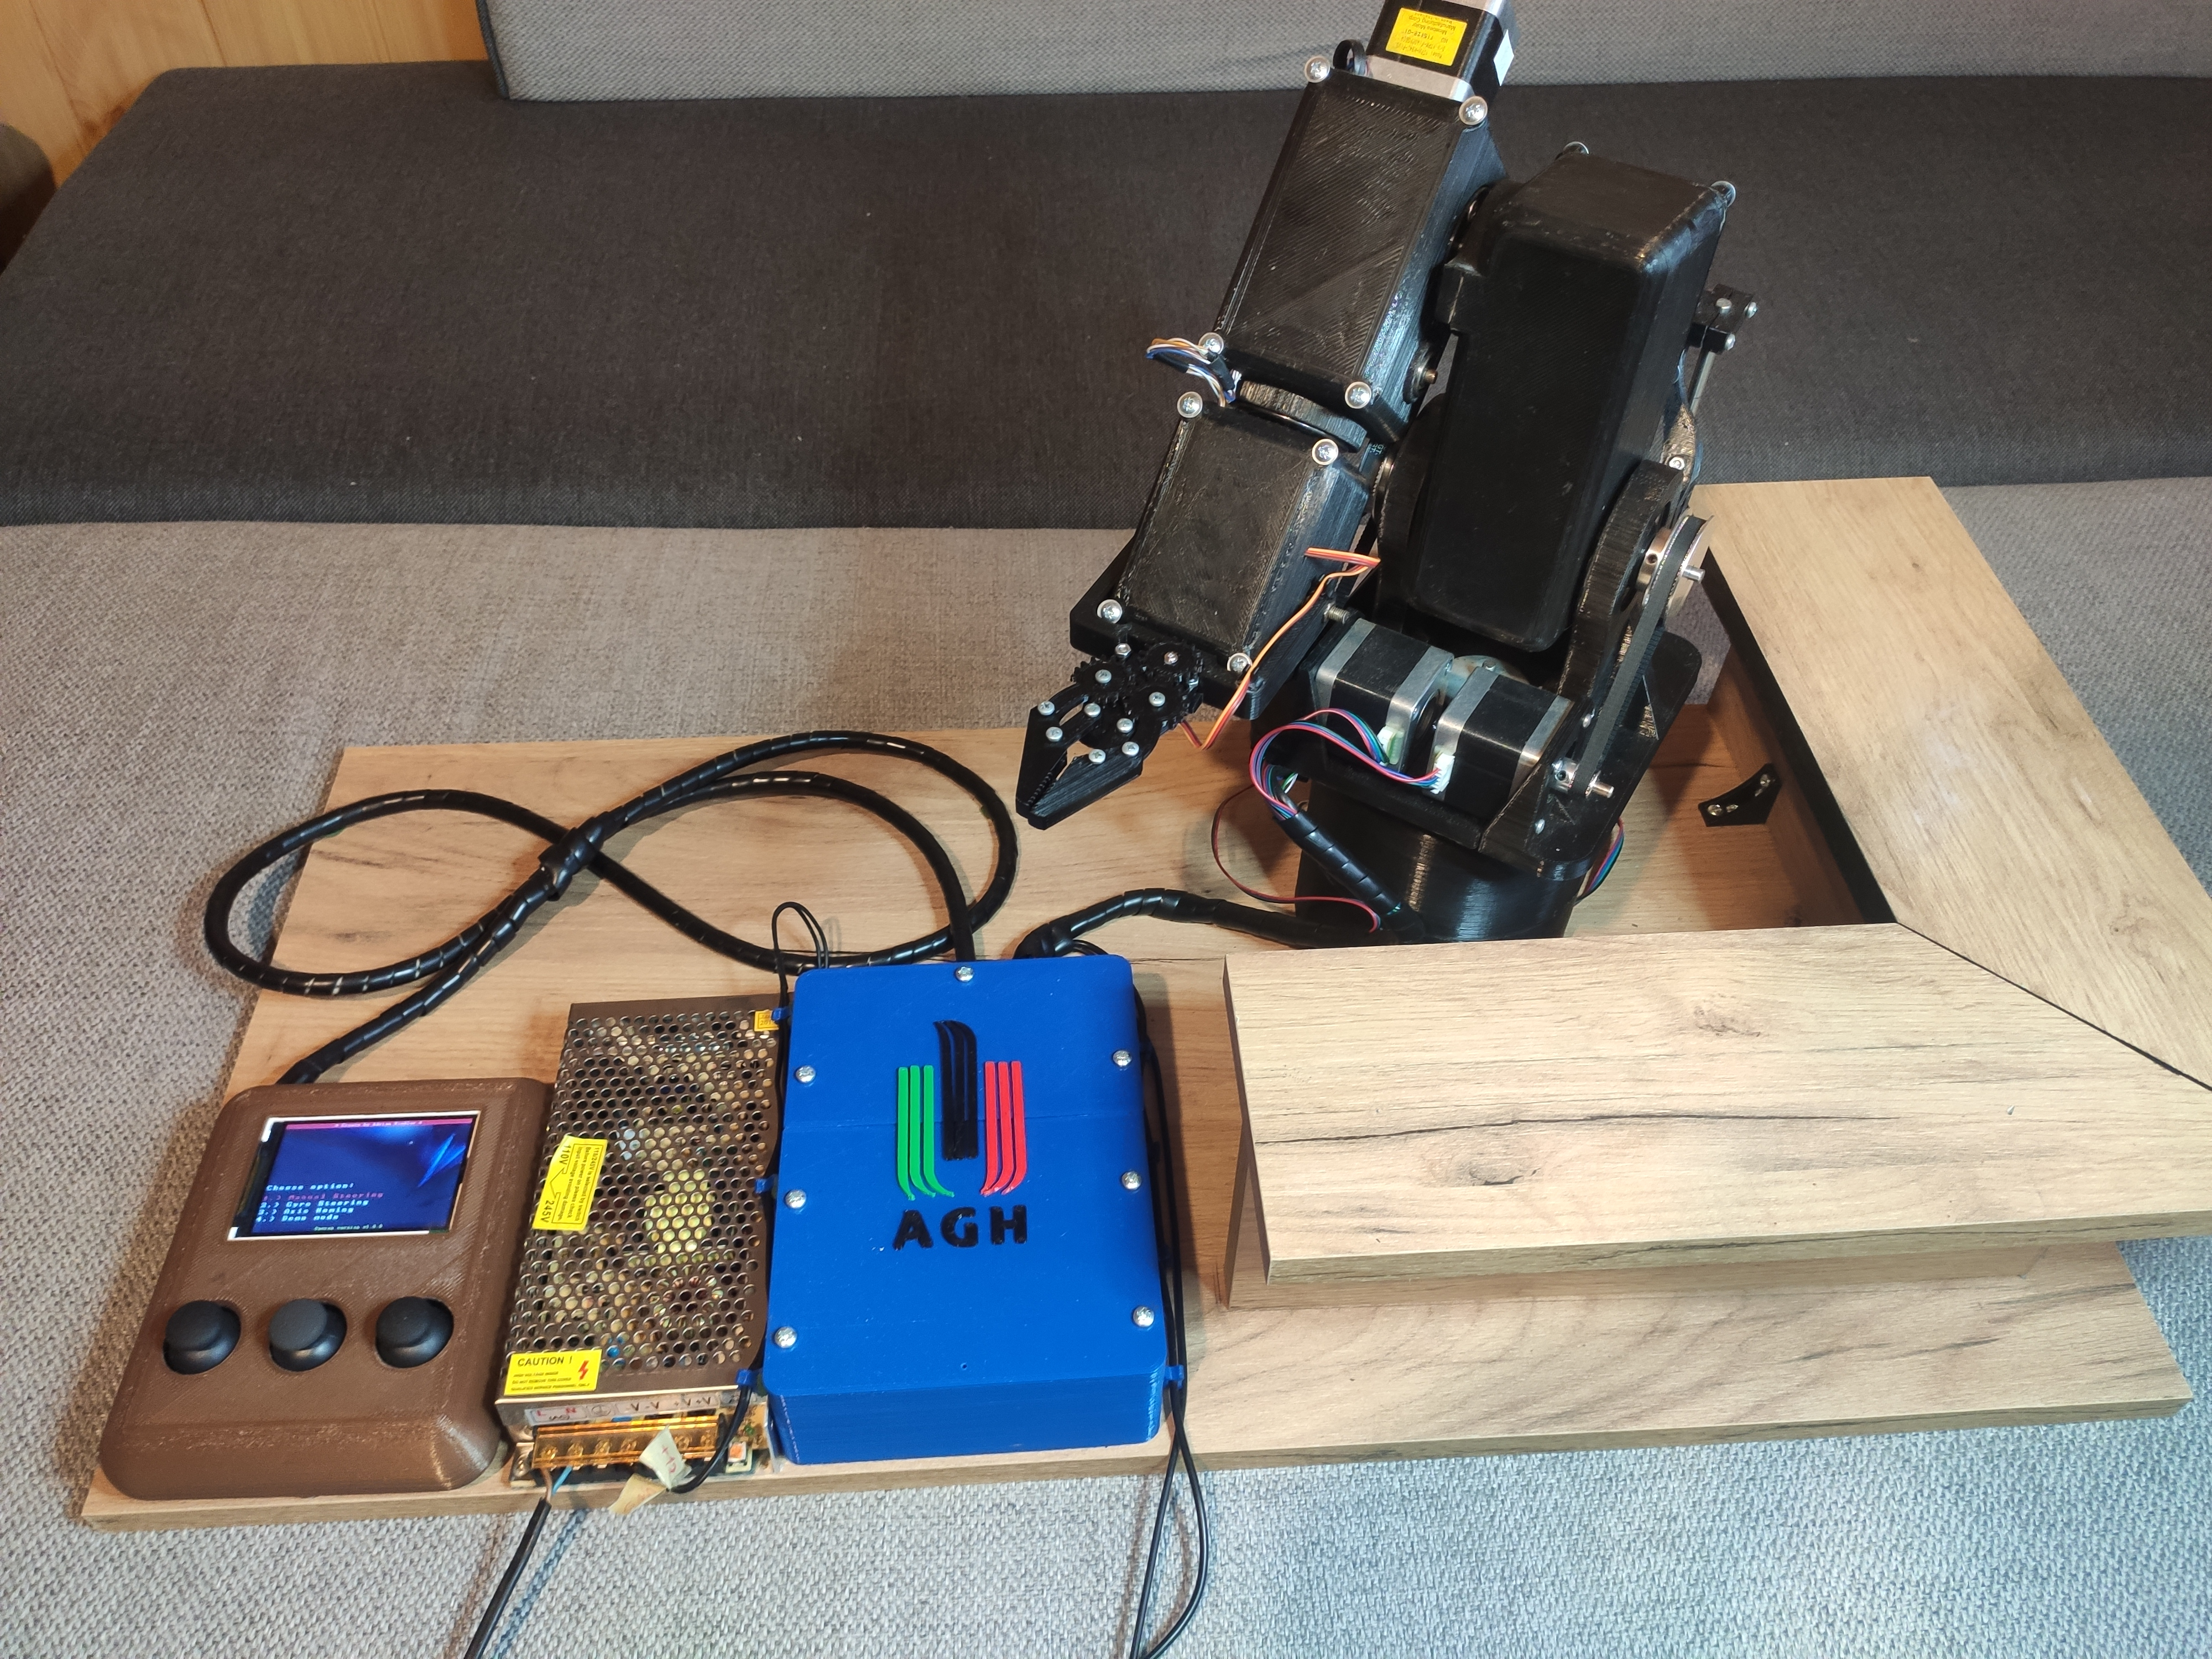
\includegraphics[width=0.9\linewidth]{{img/Bild_robot.jpg}}
	\caption{Wykorzystywany robot. \cite{own}}
	\label{fig:1}
\end{figure}

Jak można zaobserwować na poprzednim obrazie \ref{fig:1} konstrukcja wyposażona została w panel sterujący. Umożliwia on wybór jednego z trzech trybów pracy. Pierwszym z nich jest sterowanie ręczne, kiedy to użytkownik może z pomocą wbudowanych w kontroler joysticków przejąć kontrolę nad urządzeniem. Stanowiło to zarazem podstawową funkcjonalność. 

Kolejny tryb pracy związany jest z bazowaniem. Wówczas wszystkie złącza robota wracają do swoich wyjściowych pozycji. Robot został doposażony w czujniki optyczne, które po osiągnięciu przez poszczególne złącza zadanych pozycji aktywują się i tym samym informują mikrokontroler o konieczności wyłączenia silników. Funkcjonalność ta jest niezwykle istotna, gdyż po jej przeprowadzeniu urządzenie posiada informację o pozycji swoich osi. Dzięki temu możliwe jest uruchomienie trzeciego z trybów pracy manipulatora, to jest trybu demonstracyjnego. Wtedy też robot wykonuje zapisaną w oprogramowaniu sekwencję ruchów. Bazowanie jest istotne także z punktu widzenia realizowanego kontrolera ROS, gdyż pomaga w każdorazowym ustawieniu urządzenia w tej samej pozycji pierwotnej.

\section{Oprogramowanie}
\label{sec:strukturaDokumentu}

Do zrealizowania projektu wykorzystano szereg oprogramowań, które to są ze sobą mocno powiązane. Stanowią w większości swoiste rozszerzenia bądź też dodatki do głównego narzędzia jakim jest Robot Operating System - ROS. Poniżej pokrótce postanowiono omówić najważniejsze elementy wykorzystane w czasie prowadzonych działań, dla lepszego zrozumienia późniejszego powoływania się na nie.

%Oprogramowanie ROS - Robotic Operating System, składa się z wielu różnych członów funkcjonalnych, które to poniżej pokrótce opisano.

\subsection{ROS}
ROS, czyli Robot Operating System jest otwartoźródłowym oprogramowaniem, implementowanym w wszelakiej maści robotach - zarówno stacjonarnych, jak i mobilnych, na potrzeby sterowania tymi urządzeniami. Nie jest on typowym systemem operacyjnym znanym chociażby z komputerów osobisty, niemniej realizuje podobne funkcje. 
\cite{AW01}
\cite{OKa13}
ROS posiada wiele różnych dystrybucji, podobnie jak chociażby Linux. Poszczególne dystrybucje tego oprogramowania stanowią tak naprawdę jego kolejne wersje. W obrębie nich mogą występować niewielkie zmiany przy czym obejmują one funkcjonalności spoza samego rdzenia ROSa, czyli wszystko co występuje w zbiorze $ros-desktop-full$. Zmiany obejmują natomiast naprawy występujących wcześniej błędów. Istotne jest także, iż konkretne wersje ROS są dostępne dla wybranych wersji Linuxa (np. w czasie realizowania projektu ROS Noetic nie występował dla wersji Ubuntu 22.04).

To właśnie na Linuxie pracowano w czasie realizowania pracy. Co prawda na Windows 10 ROS również jest dostępny, niemniej używanie go może prowadzić do pewnych trudności.  W projekcie wykorzystywano rekomendowaną dystrybucję, jaką jest ROS Noetic. Robot Operating System jest obecnie dostępny w dwóch generacjach, ROS1 i ROS2, przy czym w projekcie wykorzystano pierwszą z nich. Powodem tej decyzji był głównie brak obecności dodatku MoveIt Setup Assistant do nowszej wersji. Dodatkowo starsza generacja posiada bardziej rozwiniętą społeczność, dzięki czemu przy debbugowaniu pojawiających się błędów łatwiej było znaleźć wsparcie w tym zakresie. \cite{ROSDoc}.

Jako iż sterowanie dowolnym robotem sprowadza się w dużej mierze do potrzeby wykorzystania podobnych mechanizmów, takich jak chociażby odczyt z czujników bądź kontrola nad silnikami, toteż ROS udostępnia szereg funkcjonalności zarządzających, łączących cały ten proces.

Istotną częścią oprogramowania ROS jest również wieloplatformowość. Ze względu na mnogość procesów składających się na całościowy system zarządzający pracą robota, nierzadko rozdziela się poszczególne zadania między różne platformy, komputery. Toteż ROS w swojej ideii udostępnia funkcjonalność upraszczającą sposób komunikowania się między systemami poprzez odpowiednie narzędzia. Zatem nie stanowi problemu uruchomienie kilku różnych instancji ROS na wielu osobnych maszynach, po czym wymienianie informacji między nimi z pomocą chociażby lokalnej sieci internetowej. Tak też poczyniono w omawianym projekcie.

Struktura ROS oparta jest zasadniczo o cztery podstawowe składowe. Pierwszą z nich stanowią tak zwane węzły (ang. $nodes$). Są to pojedyncze procesy wykonujące jedno wybrane zadanie, np. kontrolują silniki. Węzły te wymieniają między sobą informacje w sposób ciągły - poprzez tematy (ang. $topics$) bądź w sposób wywoławczy (ang. $RPC$ $-$ $Remote$ $Process$ $Call$) dzięki serwisom (ang. $services$). Podejście takie oparte na oddzielnych węzłach realizujących osobne wyszczególnione zadania niesie ze sobą pewne korzyści. Pierwszą zaletą jest spora tolerancja na błędy, ze względu na ich izolację do konkretnych węzłów. Gdy zawodzi jeden z nich to przestaje działać jedynie funkcjonalność za którą był odpowiedzialny dany węzeł, pozostałe działają nadal o ile tylko nie są zależne od tego uszkodzonego. Dywersyfikacja zadań na oddzielne procesy zmniejsza również poziom złożoności kodu. Ułatwia proces jego zrozumienia. Połączone ze sobą węzły stanowią swoisty graf. Graf taki można, dla ułatwienia zrozumienia funkcjonowania systemu podejrzeć poprzez wtyczkę wizualizującą RQT Graph. Poniżej przedstawiono obraz prezentujący zrzut ekranu z wyglądu niniejszego wizualizatora - rysunek \ref{fig:7}. Przedstawienie w ten sposób struktury ROS potrafi znacznie ułatwić pracę i zlokalizować ewentualne błędy. \cite{Nodes}

 \begin{figure}[H]
	\centering
	\includegraphics[width=0.9\linewidth]{{img/Bild_rqt.png}}
	\caption{Widok struktury węzłów i tematów ROS w RQR Graphie. \cite{own}}
	\label{fig:7}
\end{figure}

Wyżej wspomniano, iż węzły komunikują się ze sobą w sposób ciągły z wykorzystaniem tematów. Elementy te stanowią swoiste magistrale międzywęzłowe, pozwalające wymieniać wiadomości między nimi. Węzły, które publikują, generują informacje do tematów określane są mianem publisherów (ang. $publisher$), natomiast te które odbierają dane - subskrybentów (ang. $subscriber$). Tematy są zawsze jednokierunkowe, przy czym mogą mieć wielu zarówno publisherów jak i subkrybentów. Jak wspominano tematy służą do komunikacji ciągłej, realizowanej synchronicznie co ustalony kwant czasu, niemniej w przypadku informacji wysyłanych sporadycznie, od czasu do czasu - stosuje się serwisy (ang. $services$).\cite{Topics} 



W systemie rozproszonym, jaki stanowią węzły ROS czasami niezbędne jest wysłanie zapytań i odpowiedzi na nie. Taka jest zatem idea serwisów. Klient wzywa serwis poprzez wysłanie zapytania, a następnie oczekuje odpowiedzi od interesującego go węzła. Przykładowo serwis może dotyczyć wezwania węzła planującego trajektorię do rozpoczęcia tej procedury. \cite{Services}


Ostatnią z głównych składowych oprogramowania ROS są wiadomości (ang. $messages$). To na nich oparta jest komunikacja. W przypadku tematów, wiadomości stanowią struktury danych opakowujące podstawowe typy zmiennych, takie jak integer, double, boolean. Struktury te są często wielopoziomowe, zawierające nierzadko tablice zmiennych.
Natomiast rozpatrując przypadek serwisów, wówczas wiadomości przyjmują postać tak zwanych $request$ $and$ $response$ - zapytań i odpowiedzi, definiowanych w plikach $srv$ ROS. \cite{Msgs}

ROS udostępnia szereg komend, możliwych do uruchomienia z poziomu terminala komputera na którym został zainstalowany. Pozwala wywoływać pliki uruchomieniowe formatu $.launch$. Wtedy to włączane są ustalone zbiory węzłów. Umożliwia to instrukcja $roslaunch$. Możliwe jest jednak uruchomienie tylko jednego wybranego węzła z pomocą komendy $rosrun$. Obie te instrukcje cechuje identyczna składnia. Wpierw należy podać interesującą komendę - $roslaunch$ bądź $rosrun$ natomiast dalej paczkę (ang. $package$), zawierającą docelowy plik i na samym końcu właśnie nazwę pliku wykonawczego, który ma zostać uruchomiony. Istotne jest także by plikowi, który zamierza się uruchomić nadać należyte uprawnienia (instrukcja $chmod$ w Ubuntu), gdyż w przeciwnym wypadku ROS zwraca informację o nie wykrywaniu danego pliku.

Tym samym wspomniano o paczkach ROS. Programy napisane w ROS są pogrupowane w paczki, zawierające węzły, zbiory danych jak również pliki konfiguracyjne (w formcie $.yaml$) jak inne skrypty i pliki wykorzystywane przez dany zbiór. Takie paczki dostarczają konkretną funkcjonalność a jednocześnie są dosyć czytelne dla użytkowników. Ich sporą zaletą jest również duża uniwersalność, gdyż ta sama paczka może współpracować z innymi zbiorami - z czego też korzystano w realizowanym projekcie kontrolera. 

Chcąc stworzyć własny projekt w ROS, użytkownik potrzebuje przygotować opisaną wyżej paczkę. Tak też było w przypadku niniejszego projektu gdzie wygenerowana paczka stanowiła zbiór wszystkich plików zarówno symulujących jak i sterujących posiadanym robotem. 

Paczki można wygenerować automatycznie z pomocą Catkin - dedykowanego kompilatora dołączonego do ROS. Jest to istotne, gdyż każda paczka przed uruchomieniem musi zostać wpierw skompilowana z pomocą Catkina. Na tym etapie do projektu są dołączane także wykorzystywane zależności (ang. $dependencies$), czyli zbiory zewnętrznych bibliotek. Sam proces kompilacji może zająć nierzadko wiele minut, generując przy tym liczne błędy powodujące zatrzymanie się wykonywania procesu. 

\subsection{MoveIt}
MoveIt podobnie jak sam ROS jest otwartoźródłowym projektem przeznaczonym do kontrolowania robotów na poziomie planowania, manipulowania, nawigowania i percepcji trójwymiarowej. MoveIt jest swoistym rozszerzeniem, zbiorem opisywanych w poprzednim podrozdziale paczek, z którego możemy korzystać z poziomu Rviza. Struktura robota jest opisana z pomocą plików URDF. Plik ten uwzględnia geometryczne kształty urządzenia, kinematykę, punkty kolizyjne robota i inne. Dzięki temu po załadowaniu modelu, MoveIt jest w stanie dla ustalonych w pliku URDF grupy złącz robota zaplanować trajektorię ruchu. Tak by osiągnąć docelowy, zadany punkt. Realizuje on zatem zadanie liczenia kinematyki odwrotnej.  \cite{MoveitDoc},  \cite{OMPL_Mov}

\subsection{Rviz}
Rviz stanowi swoisty framework do ROS w postaci graficznego interfejsu użytkownika, w którym to wyświetlanych jest wiele przydatnych dla użytkownika informacji. Rviz pozwala na uruchamianie dodatkowych pluginów - pozwalających np. na ukazanie obrazu z zainstalowanej w robocie kamery bądź zwizualizowanie chmury punktów zwracanej przez lidar. Jak wspomniano Rviz opiera się na pluginach, które po załadowaniu zapewniają określoną przez nie funkcjonalność. Podstawowym pluginem jest $RobotModel$. Zapewnia on wizualizację posiadanego robota. Innym podstawowym pluginem jest $TF$. Zapewnia on wizualizację poszczególnych złącz w jakie zostało wyposażone posiadane urządzenie. Niemniej najistotniejszym pluginem dla rozpatrywanego projektu był właśnie MoveIt. To właśnie w interfejsie Rviz możliwe jest zadawanie pozycji robota, wybór ustawień związanych z planowaniem jak i samo planowanie i rozkazanie jego realizowania.
\cite{Rviz_rep}, \cite{Rviz}


\subsection{Gazebo}


Gazebo stanowi zaawansowane środowisko przeznaczone do symulowania zarówno samego robota jak i otoczenia w którym się znajduje. Pozwala na przetestowanie różnych scenariuszy i strategii poruszania się robota, zanim zostanie on wykorzystany w rzeczywistym projekcie. Wykorzystuje on w swoim działaniu między innymi pliki $URDF$ ($Unified$ $Robotics$ $Description$ $Format$), o których informowano już w poprzednim podroździale poświęconym narzędziu MoveIt. Mogą to być również pliki $XACRO$ bądź $SDF$, które w swojej strukturze są jednak bardzo podobne. 


Gazebo oprócz przestrzeni do symulowania zachowania się robota udostępnia również dwa dodatkowe edytory. Pierwszy z nich umożliwia tworzenie świata, przestrzeni w której użytkownik pragnąłby umieścić swoją maszynę. Natomiast drugi edytor pozwala na zbudowanie wirtualnego modelu urządzenia, a dalej wygenerować go do postaci plików $SDF$ i $config$. Dopiero na dalszym etapie z plików tych z pomocą dodatku MoveIt Setup Asisstant zostanie wygenerowany plik $URDF$. W tym miejscu należy wspomnieć, iż zdarza się, że Gazebo w czasie projektowania modelu robota zawiesza się i ostatecznie cały proces należy rozpocząć od początku. W teorii można zapisywać projekt wraz z kolejnymi etapami budowy modelu robota, niemniej w praktyce po zapisie Gazebo zmienia wszystkie dotychczasowe połączenia ramion. Dodanie kolejnego jest już wówczas bardzo utrudnione.  \cite{Gazebo}
%---------------------------------------------------------------------------

\section{Plannery}
\label{sec:kompilacja}

MoveIt zotał przystosowany do funkcjonowania z wieloma różnymi typami plannerów ścieżek i trajektorii ruchu. W poniższych podrozdziałach pokrótce opisano najważniejsze z nich. 

Pojęcie planowania stanowi kluczowy element robotyki. Jest związane z generowaniem sekwencji sterowań robota w taki sposób by uzyskać zadany ruch bądź przemieszczenie. Istnieje rozróżnienie pomiędzy zagadnieniem planowania ścieżek a planowaniem trajektorii. Czynnikiem rozróżniającym oba pojęcia jest czas. W przypadku trajektorii przemieszczenie robota uwzględnia zależność jego pozycji od konkretnej chwili ruchu. Jest zatem oparte na interpolacji funkcjami wielomianowymi. W przypadku planowania ścieżek istotne są jedynie punkty pierwotne i docelowe, bez uwzględniania pozycji urządzenia pomiędzy nimi. Ścieżki przyjmują kształty geometryczne, mogą również definiować punkty przez które ma przechodzić trasa.

\cite{Gasparetto2015}, \cite{Gasparetto2012}
\cite{MathWorks_planner}

\subsection{OMPL}

OMPL czyli The Open Motion Planning Librarry to swoisty otwartoźródłowy zbiór algorytmów planujących. Zatem biblioteka ta sama w sobie realizuje jedynie kwestie związane ze detekcją kolizji i wizualizacją. Została zaprojekotwana w taki sposób by móc zostać łatwo wykorzystana w innych programach, a jednym z nich jest właśnie wykorzystywany w projekcie MoveIt. Biblioteka OMPL w swoim zbiorze posiada sporo algorytmów planujących takich jak chociażby: PRM, RRT, EST, SBL, KPIECE, SyCLOP. \cite{OMPL}

Pierwszy z wymienionych PRM - $Probabilistic$ $Roadmap$ $Method$ jest plannerem wykorzystującym algorytm oparty na próbkowaniu. W przypadku biblioteki OMPL planner ten został zaimplementowany w oparciu o dwa wątki, gdzie jeden z nich konstruuje ścieżkę (ang. $roadmap$), natomiast drugi sprawdza czy punkty początkowe i końcowe należą do tej ścieżki. OMPL zawiera różne wariancje RPM, różniące się między sobą weryfikacją poszczególnych punktów, wierzchołków roadmapy.

RRT - $Rapidly-exploring$ $Random$ $Trees$ - kolejny dobrze znany planner oparty o algorytm próbkujący. W planerze tym każdy węzeł struktury drzewiastej (ang. $tree$ $ data$ $ structure$) generowany jest w procesie próbkowania losowego. Jak wcześniejszy posiada różne modyfikacje, z których jak najbardziej można korzystać w MoveIt. \cite{8675925}

Natomiast KPIECE - ($Kinematic$ $Planning$ $by$ $Interior-Exterior$ $Cell$ $Exploration$) jest plannerem również opartym o struktury drzewiaste, który wykorzystuje dyskretyzację wielopoziomową do prowadzenia ciągłej eksploracji przestrzeni stanów. 

\cite{MoIt_plan}

\subsection{CHOMP}

Covariant Hamiltonian optimization for motion planning (CHOMP), czyli jak wskazuje angielska definicja jest to procedura służaca planowaniu trajektorii poruszania się łańcucha kinematyczego oparta o optymalizację gradientową. Algorytm ten wykorzystuje podejście gradientowe w celu ustalenia optymalnej trajektorii. \cite{CHOMP}

\subsection{Pilz Industrial Motion Planner}

Planner ten pozwala na generowanie podstawowych trajektorii robota takich jak PTP (ang. $Point-to-Point$), LIN (ang. $Linear$) oraz CIRC (ang. $Circular$). Planner ten cechuje prostota. W zastosowaniach przemysłowych czasami konieczne jest zwykłe przemieszczenie robota w linii prostej. Takie też, bez zbędnych udziwnień dostarcza tenże planner. Nazwa algorytmu tego pochodzi od niemieckiej firmy, która jest odpowiedzialna za stworzenie tego plannera. Poprzez swą prostotę algorytm ten nie potrafi omijać przeszkód. Fakt ten został również zaobserwowany w czasie późniejszych testów. Planner ten jest jedynie generatorem ruchu, przez co właśnie po wyznaczeniu trajektorii, algorytm sprawdza czy nie występuje nigdzie kolizja. Jeżeli takowa występuje, wówczas zwraca informację o nieudanej próbie wyznaczenia trajektorii.  \cite{Pilz_AG}

%---------------------------------------------------------------------------

\section{Mikrokontrolery}
\label{sec:narzedzia}

Mikrokontrolery, których w projekcie sumarycznie wykorzystano aż cztery, są układami cyfrowymi zawartymi w jednym układzie scalonym, składającymi się z mikroprocesora i dedykowanych peryferiów. Całość pozwala na autonomiczną pracę, czyli w skrajnym przypadku do jego funkcjonowania nie jest wymagany żaden dodatkowy układ pomocniczy. Mikrokontrolery są przystosowane do pracy jako elementy sterujące bądź kontrolno-pomiarowe.

Poniżej przytoczono kilka najważniejszych informacji na temat dwóch układów o jakie rozbudowano robota na potrzeby implementacji kontrolera ROS. \cite{MiM_wyk} 

\subsection{ESP8266}

ESP8266 stanowi wysoce zintegrowany mikrokontroler wyposażony w moduł Wi-Fi, z przeznaczeniem głównie do wykorzystania w urządzeniach internetu rzeczy (ang. $Interenet$ $of$ $Things$). Głównymi zaletami są również kompaktowa budowa, niskie zużycie energii oraz wysoką efektywność.\cite{ESP_doc}


Mikrokontroler ESP8266 na potrzeby projektu programowano w języku C. Wykorzystywano w tym celu $toolchain$ do budowania aplikacji oraz $ESP8266\_RTOS\_SDK$ czyli oprogramowanie udostępniające API do ESP, a także skrypty pozwalające obsługiwać $toolchain$. Zatem sam mikrokontroler działał w oparciu o pseudosystem operacyjny FreeRTOS. Pozwalało to na napisanie w prosty sposób aplikacji wielowątkowej, co okazało się bardzo przydatne dla realizowanego zadania odczytu enkoderów. \cite{ESP_prog}

%W poniższej tabeli zamieszczono najważniejsze parametry mikrokontrolera ESP8266.


W przypadku omawianego mikrokontrolera należy również wspomnieć o konieczności dodawania do przynajmniej jednego wątku instrukcji kasującej licznik $watchdoga$. Zatem nie jest to realizowane domyślnie przez FreeRTOS, spoczywa to na barkach osoby piszącej program. Bez komendy tej urządzenie będzie się regularnie resetowało. 

Natomiast drugą kwestią jest wykorzystanie niektórych pinów GPIO. W momencie restartu mikrokontrolera, pewne wybrane piny nie mogą posiadać określonych stanów logicznych - wysokich bądź niskich, gdyż to powoduje zmianę trybu bootowania urządzenia, a przez procesor może nie chcieć się uruchomić. O ile funkcjonalność ta w pewnych przypadkach może być jak najbardziej porządna, niemniej należy mieć na uwadze takie, a nie inne zachowanie się ESP8266.

Należy również podkreślić, iż wykorzystywany w projekcie mikrokontroler ESP był w postaci płytki rozwojowej NodeMCU w wersji V3. Najważniejsze jej specyfikacje umieszczono poniżej - tabela \ref{tab:1}.

% Please add the following required packages to your document preamble:
% \usepackage[table,xcdraw]{xcolor}
% If you use beamer only pass "xcolor=table" option, i.e. \documentclass[xcolor=table]{beamer}
\begin{table}[H]
\centering
\caption{Najważniejsza specyfikacja płytki rozwojowej NodeMCU V3 \cite{ESP_param}}
\label{tab:1}
\begin{tabular}{|c|c|c|c|ll}
\cline{1-4}
\cellcolor[HTML]{C0C0C0}L.p. & \cellcolor[HTML]{C0C0C0}Parametr          & \cellcolor[HTML]{C0C0C0}Opis, wartość                          & \cellcolor[HTML]{C0C0C0}Jednostka &  &  \\ \cline{1-4}
\cellcolor[HTML]{EFEFEF}1.   & \cellcolor[HTML]{EFEFEF}Mikrokontroler    & \cellcolor[HTML]{EFEFEF}Tensilica 32-bit RISC CPU Xtensa LX106 & \cellcolor[HTML]{EFEFEF}-         &  &  \\ \cline{1-4}
\cellcolor[HTML]{C0C0C0}2.   & \cellcolor[HTML]{C0C0C0}Taktowanie zegara & \cellcolor[HTML]{C0C0C0}80                                     & \cellcolor[HTML]{C0C0C0}MHz       &  &  \\ \cline{1-4}
\cellcolor[HTML]{EFEFEF}3.   & \cellcolor[HTML]{EFEFEF}Napięcie pracy    & \cellcolor[HTML]{EFEFEF}3.3                                    & \cellcolor[HTML]{EFEFEF}V         &  &  \\ \cline{1-4}
\cellcolor[HTML]{C0C0C0}4.   & \cellcolor[HTML]{C0C0C0}Pamięć Flash      & \cellcolor[HTML]{C0C0C0}4                                      & \cellcolor[HTML]{C0C0C0}MB        &  &  \\ \cline{1-4}
\cellcolor[HTML]{EFEFEF}5.   & \cellcolor[HTML]{EFEFEF}Pamięć SRAM       & \cellcolor[HTML]{EFEFEF}128                                    & \cellcolor[HTML]{EFEFEF}KB        &  &  \\ \cline{1-4}
\cellcolor[HTML]{C0C0C0}6.   & \cellcolor[HTML]{C0C0C0}Ilość pinów GPIO  & \cellcolor[HTML]{C0C0C0}17                                     & \cellcolor[HTML]{C0C0C0}-         &  &  \\ \cline{1-4}
\cellcolor[HTML]{EFEFEF}7.   & \cellcolor[HTML]{EFEFEF}Wbudowane WiFi    & \cellcolor[HTML]{EFEFEF}802.11 b/g/n                           & \cellcolor[HTML]{EFEFEF}-         &  &  \\ \cline{1-4}
\cellcolor[HTML]{C0C0C0}8.   & \cellcolor[HTML]{C0C0C0}Magistrale        & \cellcolor[HTML]{C0C0C0}UART/I2C/SPI                           & \cellcolor[HTML]{C0C0C0}-         &  &  \\ \cline{1-4}
\cellcolor[HTML]{EFEFEF}9.   & \cellcolor[HTML]{EFEFEF}Przetworniki      & \cellcolor[HTML]{EFEFEF}Jeden ADC                              & \cellcolor[HTML]{EFEFEF}-         &  &  \\ \cline{1-4}
\end{tabular}
\end{table}

\subsection{Raspberry Pi4B}

Raspberry Pi 4B stanowił w momencie pisania niniejszej pracy najnowsze wydanie popularnej serii mikrokomputerów brytyjskiej organizacji Raspberry Pi Foundation. Urządzenie to oprócz dostarczania podstawowej funkcjonalności spotykanej w komputerach klasy PC, udostępnia użytkownikowi również 28 pinów GPIO (ang. $General$ $Purpose$ $Input$ $Output$) - podobnie jak klasyczny mikrokontroler. Najważniejsze parametry mikrokomputera RPI4B wymieniono w poniższej tabeli \ref{tab:2}.


\begin{table}[H]
\centering
\caption{Najważniejsza specyfikacja mikrokomputera Raspberry Pi4B \cite{RPI_par}}
\label{tab:2}
\begin{tabular}{|c|c|c|c|ll}
\cline{1-4}
\cellcolor[HTML]{C0C0C0}L.p. & \cellcolor[HTML]{C0C0C0}Parametr          & \cellcolor[HTML]{C0C0C0}Opis, wartość                   & \cellcolor[HTML]{C0C0C0}Jednostka &  &  \\ \cline{1-4}
\cellcolor[HTML]{EFEFEF}1.   & \cellcolor[HTML]{EFEFEF}Procesor          & \cellcolor[HTML]{EFEFEF}Quad core 64-bit ARM-Cortex A72 & \cellcolor[HTML]{EFEFEF}-         &  &  \\ \cline{1-4}
\cellcolor[HTML]{C0C0C0}2.   & \cellcolor[HTML]{C0C0C0}Taktowanie zegara & \cellcolor[HTML]{C0C0C0}1.5                             & \cellcolor[HTML]{C0C0C0}GHz       &  &  \\ \cline{1-4}
\cellcolor[HTML]{EFEFEF}3.   & \cellcolor[HTML]{EFEFEF}Pamięć RAM        & \cellcolor[HTML]{EFEFEF}2, 4, 8 (w projekcie użyto 8)   & \cellcolor[HTML]{EFEFEF}GB        &  &  \\ \cline{1-4}
\cellcolor[HTML]{C0C0C0}4.   & \cellcolor[HTML]{C0C0C0}Bluetooth         & \cellcolor[HTML]{C0C0C0}5.0 z Bluetooth Low Energy      & \cellcolor[HTML]{C0C0C0}-         &  &  \\ \cline{1-4}
\cellcolor[HTML]{EFEFEF}5.   & \cellcolor[HTML]{EFEFEF}Wbudowane WiFi    & \cellcolor[HTML]{EFEFEF}802.11 b/g/n/ac                 & \cellcolor[HTML]{EFEFEF}-         &  &  \\ \cline{1-4}
\cellcolor[HTML]{C0C0C0}6.   & \cellcolor[HTML]{C0C0C0}Ilość pinów GPIO  & \cellcolor[HTML]{C0C0C0}28 (w tym PWM i GPCLK)          & \cellcolor[HTML]{C0C0C0}sztuk     &  &  \\ \cline{1-4}
\cellcolor[HTML]{EFEFEF}7.   & \cellcolor[HTML]{EFEFEF}Porty USB         & \cellcolor[HTML]{EFEFEF}2 x 2.0 i 2 x 3.0               & \cellcolor[HTML]{EFEFEF}sztuki    &  &  \\ \cline{1-4}
\cellcolor[HTML]{C0C0C0}8.   & \cellcolor[HTML]{C0C0C0}Magistrale        & \cellcolor[HTML]{C0C0C0}UART/I2C/SPI/SDIO/DPI/PCM       & \cellcolor[HTML]{C0C0C0}-         &  &  \\ \cline{1-4}
\cellcolor[HTML]{EFEFEF}9.   & \cellcolor[HTML]{EFEFEF}Porty micro-HDMI  & \cellcolor[HTML]{EFEFEF}2                               & \cellcolor[HTML]{EFEFEF}sztuki    &  &  \\ \cline{1-4}
\cellcolor[HTML]{C0C0C0}10.  & \cellcolor[HTML]{C0C0C0}Port SD Card      & \cellcolor[HTML]{C0C0C0}1                               & \cellcolor[HTML]{C0C0C0}sztuka    &  &  \\ \cline{1-4}
\end{tabular}
\end{table}

 Wszystkie te parametry sprawiają, iż układ w pewnym stopniu może nawet zastąpić komputer osobisty. O ile użytkowanie go jako urządzenie multimedialne, mimo iż jest to możliwe, to jest to raczej mało praktyczne, o tyle wykorzystanie w projektach podobnych do opisywanego w niniejszej pracy jest jak najbardziej wskazane. W takich sytuacja oferowana moc obliczeniowa jest wystarczająca.

Jako iż Raspberry posiada w swojej budowie piny GPIO, toteż teoretycznie, sam ten mikrokomputer mógłby być wykorzystywany do obsługi zarówno enkoderów, czujników jak i do sterowania silnikami krokowymi robota. Zatem dwa dodatkowe mikrokontrolery STM oraz ESP mogą wydawać się naddatkowe. Niemniej realizując projekt zamierzano rozszerzyć obecną funkcjonalność a nie ją zastępować. Toteż nie chciano porzucać już wypracowanych rozwiązań. Natomiast drugą kwestią, możliwe że nawet istotniejszą jest kwestia zabezpieczenia mikrokomputera Raspberry Pi przed uszkodzeniem. W czasie realizacji projektu inżynierskiego, w czasie prób, uszkodzono pierwotny mikrokontroler STM32 (doprowadzając przez przypadek do zwarcia), toteż chcąc nie dopuścić do podobnej sytuacji w przypadku RPI4B postanowiono nie instalować go w miejsce STM32, tylko połączyć z nim poprzez przewód USB.


%---------------------------------------------------------------------------

\section{Podsumowanie rozdziału}

Podsumowując niniejszy rozdział, można napisać, iż co prawda projekt łączy w sobie wiele różnych zagadnień, niemniej starano się je w sposób zwięzły i zrozumiały przytoczyć. Wiele kwestii zostało znacznie spłyconych i przez to okrojonych, niemniej np. tematyka plannerów jest tak złożona, iż prawdopodobnie zagłębianie się w szczegóły mogłoby mijać się z celem. Są to tematy poruszane przez wiele artykułów naukowych, planowanie optymalnej ścieżki, w możliwie najkrótszym czasie, z uwzględnieniem towarzyszących robotowi przeszkód stanowi problem badawczy, którym zajmują się naukowcy z całego świata. Celem projektu było między innymi porównanie tychże plannerów w swoim działaniu pomiędzy sobą, natomiast mniej analizowanie dokładnie mechaniki na której się opierają.

W rozdziale tym starano się też wspominać o pewnych kwestiach, które okazują się przydatne przy bezpośredniej implementacji zadań, tak jak to miało chociażby miejsce w przypadku ESP8266 - wspominając o jego zachowaniu przy restarcie. Wiedza taka może zaoszczędzić sporo czasu.

\label{sec:przygotowanieDokumentu}

